
%%%%%%%%%%%%%%%%%%%%%%%%%%%%%%%%%%%%%%%%%%%%%%%%%%%%%%%%%%%%%%



\section{Introdução}
\begin{frame}

    \frametitle{Histórico}

    \begin{itemize}
      \item Criada em 2013 por Neng-Fa Zhou e Jonathan Fruhman 

      \item Utiliza o B-Prolog como base de implementação, e ambas utilizam 
      a  programação em lógica: Lógica de Primeira-Ordem (LPO)

      \item Uma evolução ao Prolog após seus mais de 40 anos de sucesso!

      \item Sua atual versão é a 2.0 (\today)

    \end{itemize}
\end{frame}

%%%%%%%%%%%%%%%%%%%%%%%%%%%%%%%%%%%%%%%%%%%%%%%%%%%%%%%%%%%%%%%%%%%%%

%\section{Isso é outra seção}
\begin{frame}
    \frametitle{O que é multiparadigma?}

    \begin{itemize}
      \item Imperativo -- Procedural
      \item Funcional
      \item \underline{Lógico}
      \item Uma boa \textit{mistura} de: Haskell, Prolog e Python

    \end{itemize}

\end{frame}

%%%%%%%%%%%%%%%%%%%%%%%%%%%%%%%%%%%%%%%%%%%%%%%%%%%%%%%%%%%%%%%%%%%%%

\begin{frame}
    \frametitle{Algumas Características:}

    \begin{itemize}
    
      \item Sintaxe $\Rightarrow $ elegância do código
      \item Velocidade de execução
      \item Portabilidade (todas plataformas)
      \item Extensão há outras ferramentas
      
    \end{itemize}
\end{frame}

%%%%%%%%%%%%%%%%%%%%%%%%%%%%%%%%%%%%%%%%%%%%%%%%%%%%%%%%%%%%%%%%%%%%%


%%%%%%%%%%%%%%%%%%%%%%%%%%%%%%%%%%%%%%%%%%%%%%%%%%%%%%%%%%%%%%%%%%%%%

\section{Características}
\begin{frame}
    \frametitle{Anacrônico de \textbf{P.I.C.A.T.}}
  
 \begin{description}
   
 
 \item [\textbf{P}:] \textit{Pattern-matching}:  Utiliza o conceito de \textit{casamento padrão}
 equivalente aos conceitos de \textit{unificação} da LPO
 
 \item [\textbf{I}:] \textit{Intuitive}: oferece estruturas de decisão, atribuição e 
 laços de repetição, etc, análogo as outras linguagens de programação
 
  \item [\textbf{C}:] \textit{Constraints}: suporta a Programação por Restrições (PR)
 
     \item [\textbf{A}:] \textit{Actors}: suporte as chamadas a eventos, os atores (futuro gráfico) 
 
  \item [\textbf{T}:] \textit{Tabling}: implementa a técnica de \textit{memoization}, com soluções imediatas para problemas de Programação Dinâmica (PD).
   
  
\end{description}
\end{frame}

%%%%%%%%%%%%%%%%%%%%%%%%%%%%%%%%%%%%%%%%%%%%%%%%%%%%%%%%%%%%%%%%%%%%%

%%%%%%%%%%%%%%%%%%%%%%%%%%%%%%%%%%%%%%%%%%%%%%%%%%%%%%%%%%%%%%%%%%%%%
\subsection{Instalação}
\begin{frame}
    \frametitle{Instalação do PICAT}

  \begin{itemize}
    \item Baixar a versão desejada de \url{http://picat-lang.org/download.html}
   \item Descompactar. Em geral em \textbf{/usr/local/Picat/}
    \item Criar um link simbólico (linux) ou atalhos (Windows):\\ 
   \texttt{ln -s /usr/local/Picat/picat   \hspace{1cm}   /usr/bin/picat}
    \item Se quiser adicionar (opcional) uma variável de ambiente:\\
          \texttt{PICATPATH=/usr/local/Picat/}\\
          \texttt{export PICATPATH}

    \item ou ainda adicione o caminho: \texttt{PATH=\$PATH:/usr/local/Picat}

   \item Finalmente, tenha um editor de código de programa.\\
     Sugestão: \textit{geany} ou \textit{sublime}
     
    \item Escolha a sintaxe da linguagem \textit{Erlang} 
    
  \end{itemize}



\end{frame}

%%%%%%%%%%%%%%%%%%%%%%%%%%%%%%%%%%%%%%%%%%%%%%%%%%%%%%%%%%%%%%%%%%%%%


%%%%%%%%%%%%%%%%%%%%%%%%%%%%%%%%%%%%%%%%%%%%%%%%%%%%%%%%%%%%%%%%%%%%%
\subsection{Usando do Picat}

\begin{frame}
    \frametitle{Usando do Picat}
    \begin{itemize}
     \item Picat é uma linguagem de multiplataforma, disponível em qualquer arquitetura de processamento e também de sistema operacional. Nesta vídeo-aula: Linux (Manjaro)
     \item Em seus arquivos fontes utiliza a extensão \textbf{.pi}. Exemplo: \texttt{programa.pi}
     \item Existem 2 modos de utilização do Picat: modo linha de comando (ou console) e modo interativo
     \item Códigos executáveis 100\% \textbf{stand-alone}: ainda não!
     \item Neste quesito, estamos em igualdade com Java, Prolog e Python
     
    \end{itemize}
\end{frame}

%%%%%%%%%%%%%%%%%%%%%%%%%%%%%%%%%%%%%%%%%%%%%%%%%%%%%%%%%%%%%%%%%%%%%

%%%%%%%%%%%%%%%%%%%%%%%%%%%%%%%%%%%%%%%%%%%%%%%%%%%%%%%%%%%%%%%%%%%%%
\section{Exemplo}
\begin{frame}
    \frametitle{Fatos e Regras -- os pais!}
    \begin{itemize}
    
    \item $pai(platao, luna)$ \hspace{1.5cm} leia-se: \textit{Platão é o pai de Luna}
    \item $pai(platao, péricles)$ \hspace{1.5cm} leia-se: \textit{Platão é o pai de Péricles}
    \item $pai(epimenides, platao)$ \hspace{1.5cm} leia-se: \textit{Sócrates é o pai de Platão}
    \item Codificando tudo isto  em Picat
    \end{itemize}
\end{frame}

\begin{frame}[allowframebreaks=0.9]
 \frametitle{Regras em PICAT}

\lstinputlisting{../regras_ex_02.pi}

\end{frame}


%%%%%%%%%%%%%%%%%%%%%%%%%%%%%%%%%%%%%%%%%%%%%%%%%%%%%%%%%%%%%%%%%%%%%

\section{Tipos de Dados}

\begin{frame}
\frametitle{Tipos de Dados}
\begin{figure}[!ht]
\centering
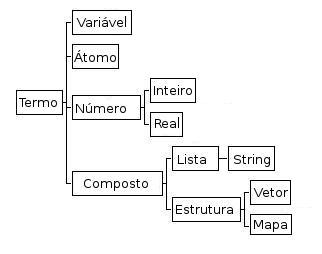
\includegraphics[width=.6\textwidth]{figures/tipos_dados_picat_traduzido.jpg}
\caption{Hierarquia dos Tipos de dados}
\label{Hiera}
\end{figure}
\end{frame}

%%%%%%%%%%%%%%%%%%%%%%%%%%%%%%%%%%%%%%%%%%%%%%%%%%%%%%%%%%%%%%%%%%%%%

%%%%%%%%%%%%%%%%%%%%%%%%%%%%%%%%%%%%%%%%%%%%%%%%%%%%%%%%%%%%%%%%%%%%%
\subsection{Outros Detalhes}
\begin{frame}
    \frametitle{Número}
    \texttt{Picat> A = 5, B = 7, number(A), number(B),
    max(A, B) = Maximo, min(A, B) = Minimo.}\\
  
    \texttt{A = 5}\\
    \texttt{B = 7}\\
    \texttt{Maximo = 7}\\
    \texttt{Minimo = 5}\\
    \texttt{yes.}
\end{frame}

%%%%%%%%%%%%%%%%%%%%%%%%%%%%%%%%%%%%%%%%%%%%%%%%%%%%%%%%%%%%%%%%%%%%%


%%%%%%%%%%%%%%%%%%%%%%%%%%%%%%%%%%%%%%%%%%%%%%%%%%%%%%%%%%%%%%%%%%%%%


%%%%%%%%%%%%%%%%%%%%%%%%%%%%%%%%%%%%%%%%%%%%%%%%%%%%%%%%%%%%%%%%%%%%%

\begin{frame}
    \frametitle{Atribuição}
     \texttt{Picat> X := 7, X := X + 7, X := X + 7.}\\
     \texttt{X = 21}
\end{frame}

%%%%%%%%%%%%%%%%%%%%%%%%%%%%%%%%%%%%%%%%%%%%%%%%%%%%%%%%%%%%%%%%%%%%%

\begin{frame}
    \frametitle{Estruturas de Controle}
        
     \lstinputlisting{../estrutura_if_then_ex01.pi}
    
\end{frame}

%%%%%%%%%%%%%%%%%%%%%%%%%%%%%%%%%%%%%%%%%%%%%%%%%%%%%%%%%%%%%%%%%%%%%

\begin{frame}
    \frametitle{Entradas e Saídas}
  
  
  \lstinputlisting{../media_2_reais.pi}
  
\end{frame}
%%%%%%%%%%%%%%%%%%%%%%%%%%%%%%%%%%%%%%%%%%%%%%%%%%%%%%%%%%%%%%%%%%%%%

%%%%%%%%%%%%%%%%%%%%%%%%%%%%%%%%%%%%%%%%%%%%%%%%%%%%%%%%%%%%%%%%%%%%%

%%%%%%%%%%%%%%%%%%%%%%%%%%%%%%%%%%%%%%%%%%%%%%%%%%%%%%%%%%%%%%%%%%%%%
%%%%%%%%%%%%%%%%%%%%%%%%%%%%%%%%%%%%%%%%%%%%%%%%%%%%%%%%%%%%%%%%%

\section{Conclusão}
\begin{frame}
    \frametitle{Conclusão}
    \begin{itemize}
    \item PICAT é uma linguagem nova (2013), 
    desconhecida, revolucionária e com um futuro promissor
    
    \item Atualmente há pouco material disponível e uma comunidade pequena de usuários

    \item Uso muito bom quanto a: Planejamento, Programação por Restrição e PD (diretamente)
    
    \item Todos problemas NPs-Completos!
    \end{itemize}
\end{frame}

%%%%%%%%%%%%%%%%%%%%%%%%%%%%%%%%%%%%%%%%%%%%%%%%%%%%%%%%%%%%%%%%%%%%%

%\section{Referências}
\begin{frame}
    \frametitle{Referências}
    \begin{itemize}
    \item O \textit{User Guide} que está no diretório  \texttt{doc/} da instalação em \LaTeX
    
     \item Meu GitHub $\Rightarrow $  \url{https://github.com/claudiosa/CCS/tree/master/picat}

     \item \url{http://pic at-lang.org/} -- \textit{User Guide on-line} está lá
    
    \item Assinem o fórum do PICAT(em inglês: respondo lá também)

    \item Site do Hakan  Kjellerstrand  $\Rightarrow $ \url{http://www.hakank.org/picat/}
    \item Site do Roman Barták  $\Rightarrow $ 	\url{http://ktiml.mff.cuni.cz/~bartak/}
    \item Site do Sergii Dimychenko  $\Rightarrow $ \url{http://sdymchenko.com/blog/2015/01/31/ai-planning-picat/}
    
    \end{itemize}
\end{frame}

%%%%%%%%%%%%%%%%%%%%%%%%%%%%%%%%%%%%%%%%%%%%%%%%%%%%%%%%%%%%%%%%%%%%%
